% !TeX root = ../SDonchezThesis.tex

\appendix

\chapter{EDF Development Container Specification}\label{apx:EDFDocker}
\begin{lstlisting}[language=docker, breaklines=true, caption={Dockerfile for EDF Development Container}, label=lst:Dockerfile]
FROM ubuntu:18.04

# build with "docker build --build-arg PETA_VERSION=2020.2 --build-arg PETA_RUN_FILE=petalinux-v2020.2-final-installer.run -t petalinux:2020.2 ."

# install dependences:

ARG UBUNTU_MIRROR
RUN [ -z "${UBUNTU_MIRROR}" ] || sed -i.bak s/archive.ubuntu.com/${UBUNTU_MIRROR}/g /etc/apt/sources.list 

RUN apt-get update &&  DEBIAN_FRONTEND=noninteractive apt-get install -y -q \
  build-essential \
  sudo \
  tofrodos \
  iproute2 \
  gawk \
  net-tools \
  expect \
  libncurses5-dev \
  update-inetd \
  libssl-dev \
  flex \
  bison \
  libselinux1 \
  gnupg \
  wget \
  socat \
  gcc-multilib \
  libidn11 \
  libsdl1.2-dev \
  libglib2.0-dev \
  lib32z1-dev \
  libgtk2.0-0 \
  libtinfo5 \
  xxd \
  screen \
  pax \
  diffstat \
  xvfb \
  xterm \
  texinfo \
  gzip \
  unzip \
  cpio \
  chrpath \
  autoconf \
  lsb-release \
  libtool \
  libtool-bin \
  locales \
  kmod \
  git \
  rsync \
  bc \
  u-boot-tools \
  python \
  xinetd \
  tftpd \
  tftp \
  libsm6 \
  libxi6 \
  libxrandr2 \
  libfreetype6 \
  libfontconfig \
  libswt-gtk-4-java \
 && apt-get clean \
 && rm -rf /var/lib/apt/lists/*

RUN dpkg --add-architecture i386 &&  apt-get update &&  \
      DEBIAN_FRONTEND=noninteractive apt-get install -y -q \
      zlib1g:i386 \
    && apt-get clean \
    && rm -rf /var/lib/apt/lists/*

ARG PETA_RUN_FILE
ARG VIVADO_TAR_FILE
ARG VIVADO_VERSION

RUN locale-gen en_US.UTF-8 && update-locale

#make a Vivado user
RUN adduser --disabled-password --gecos '' vivado && \
  usermod -aG sudo vivado && \
  echo "vivado ALL=(ALL) NOPASSWD: ALL" >> /etc/sudoers

COPY .devcontainer/accept-eula.sh /tmp/
COPY .devcontainer/${VIVADO_TAR_FILE}.tar.gz /
COPY .devcontainer/install_config_vitis.txt /
COPY .devcontainer/install_config_petalinux.txt /

#config tftp server
COPY .devcontainer/tftp.in /etc/xinetd.d/tftp
RUN mkdir /tftpboot
RUN chmod ugo+rw /tftpboot/
RUN service xinetd stop
RUN service xinetd start

# run the install

RUN echo "Extracting Vivado tar file" 
RUN tar xzf ${VIVADO_TAR_FILE}.tar.gz 
RUN rm ${VIVADO_TAR_FILE}.tar.gz
RUN ${VIVADO_TAR_FILE}/xsetup --agree 3rdPartyEULA,WebTalkTerms,XilinxEULA --batch Install --config install_config_vitis.txt 
RUN ${VIVADO_TAR_FILE}/xsetup --agree 3rdPartyEULA,WebTalkTerms,XilinxEULA --batch Install --config install_config_petalinux.txt
RUN mkdir /tools/Xilinx/PetaLinux/${VIVADO_VERSION}/install/
RUN chmod -R 777 /tools/Xilinx/PetaLinux/${VIVADO_VERSION}/
RUN chmod -R 777 /tmp/
RUN cd /tmp && \
  sudo -u vivado -i /tmp/accept-eula.sh /tools/Xilinx/PetaLinux/${VIVADO_VERSION}/bin/${PETA_RUN_FILE} /tools/Xilinx/PetaLinux/${VIVADO_VERSION}/install/
RUN rm -f /tools/Xilinx/PetaLinux/${VIVADO_VERSION}/bin/${PETA_RUN_FILE} /tmp/accept-eula.sh
RUN rm -rf ${VIVADO_TAR_FILE}*

# make /bin/sh symlink to bash instead of dash:
RUN echo "dash dash/sh boolean false" | debconf-set-selections
RUN DEBIAN_FRONTEND=noninteractive dpkg-reconfigure dash

USER vivado
ENV HOME /home/vivado
ENV LANG en_US.UTF-8

#add vivado tools to path
RUN echo "service xinetd start" >> /home/vivado/.bashrc
RUN echo "source /tools/Xilinx/Vitis/2020.2/settings64.sh" >> /home/vivado/.bashrc
RUN echo "source /tools/Xilinx/PetaLinux/2020.2/install/settings.sh" >> /home/vivado/.bashrc

#setup vivado license
RUN mkdir /home/vivado/.Xilinx
COPY .devcontainer/Xilinx.lic /home/vivado/.Xilinx/
\end{lstlisting}


\chapter{XMPU-PL Design (enlarged)}\label{apx:xmpu-pl-design-enlarged}
\begin{figure}
  \centering
  %TODO: make larger somehow
    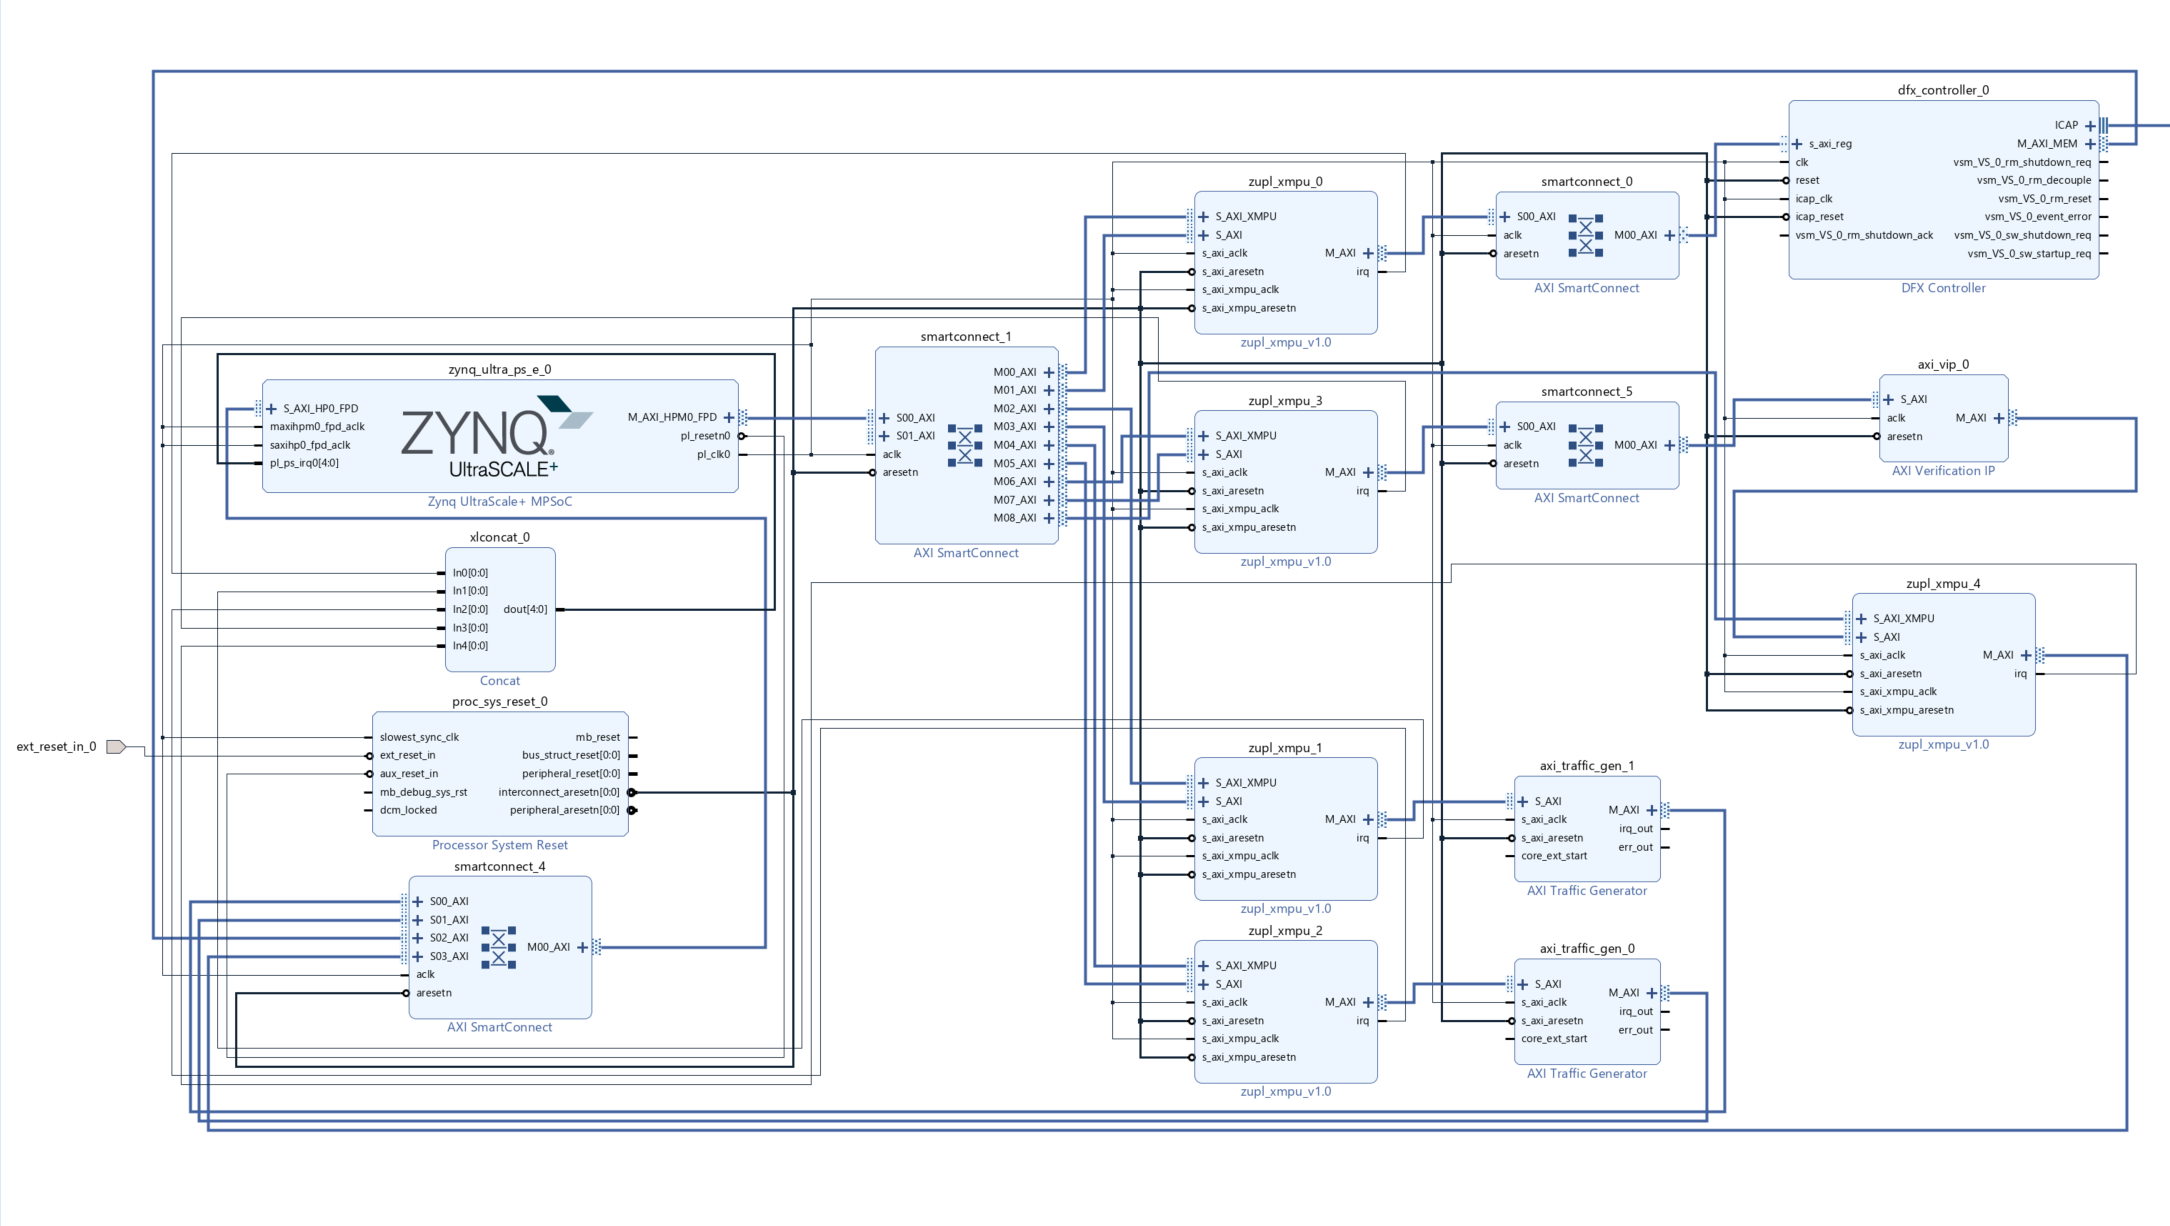
\includegraphics[width=\textwidth,height=\textheight,keepaspectratio,angle=90]{isolation_bd.png}
    \caption [Proposed XMPU-PL Design (enlarged)]{Xilinx Memory Protection Unit for Programmable Logic (XMPU-PL) in a Zynq UltraScale+ MPSoC architecture (enlarged)}
    \label{fig:XMPU-PLDesign_large}
\end{figure}